%% fig_fibres.tex   (generated by make_plates.py; do not edit by hand)
%% Lemma lem:annihilator at n = 3: the basis of wedge^2 H^{0,1} in three blocks, the mixed block the kernel of multiplication by omega; and the three dimensions for n = 2, ..., 6.
\documentclass[tikz,border=6pt]{standalone}
\usepackage{amsmath,amssymb}
\usetikzlibrary{arrows.meta,calc,patterns,decorations.pathreplacing}
%% palette.tex -- shared colour definitions for the figures
\definecolor{PInk}{RGB}{26,32,44}
\definecolor{PBlue}{RGB}{37,82,139}
\definecolor{PTeal}{RGB}{23,127,125}
\definecolor{POchre}{RGB}{193,138,44}
\definecolor{PClay}{RGB}{178,74,58}
\definecolor{PSlate}{RGB}{108,122,137}
\definecolor{PViolet}{RGB}{110,86,150}
\definecolor{WBlue}{RGB}{223,234,246}
\definecolor{WTeal}{RGB}{220,238,236}
\definecolor{WOchre}{RGB}{250,240,218}
\definecolor{WClay}{RGB}{247,229,224}
\definecolor{WSlate}{RGB}{238,241,244}
\definecolor{PMag}{RGB}{158,58,110}
\definecolor{PGrass}{RGB}{62,124,66}
\definecolor{PAmber}{RGB}{214,112,38}
\definecolor{PIndigo}{RGB}{58,64,140}
\definecolor{PRule}{RGB}{176,186,197}

%% shared macros so the standalone figures match the paper
\providecommand{\QQ}{\mathbb{Q}}
\providecommand{\ZZ}{\mathbb{Z}}
\providecommand{\RR}{\mathbb{R}}
\providecommand{\CC}{\mathbb{C}}
\providecommand{\PP}{\mathbb{P}}
\providecommand{\Kx}{K^{\times}}
\providecommand{\HW}{W}
\providecommand{\Nm}{\mathrm{N}}
\providecommand{\Hdg}{\mathrm{Hdg}}
\providecommand{\NS}{\mathrm{NS}}
\providecommand{\cA}{\mathcal{A}}
\providecommand{\cD}{\mathcal{D}}
\providecommand{\cF}{\mathcal{F}}
\providecommand{\cP}{\mathcal{P}}
\providecommand{\cO}{\mathcal{O}}
\providecommand{\cQ}{\mathcal{Q}}
\providecommand{\bbar}[1]{\overline{#1}}
\providecommand{\ch}{\operatorname{ch}}
\providecommand{\End}{\mathrm{End}}
\providecommand{\Ext}{\operatorname{Ext}}
\providecommand{\Supp}{\operatorname{Supp}}

\begin{document}
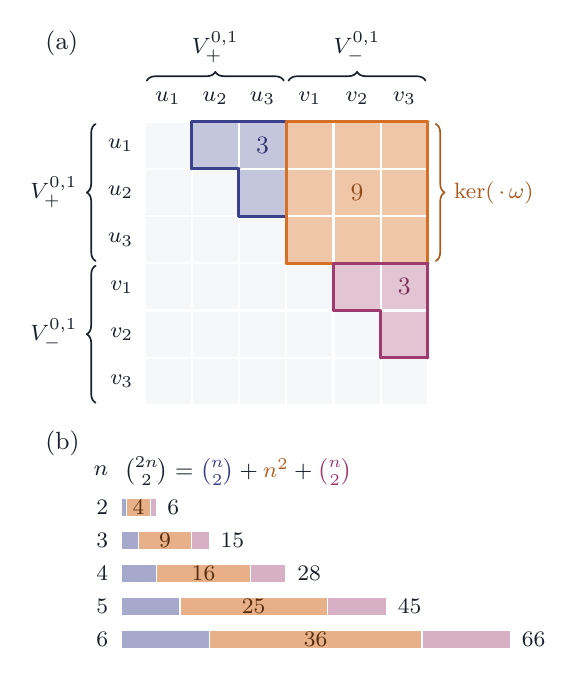
\begin{tikzpicture}[x=1cm,y=1cm,line join=round,line cap=round,
  font=\small,text=PInk]
  \filldraw[WSlate!55,draw=white,line width=0.80pt] (1.300,6.900) -- (1.900,6.900) -- (1.900,7.500) -- (1.300,7.500) -- cycle;
  \filldraw[PIndigo!30,draw=white,line width=0.80pt] (1.900,6.900) -- (2.500,6.900) -- (2.500,7.500) -- (1.900,7.500) -- cycle;
  \filldraw[PIndigo!30,draw=white,line width=0.80pt] (2.500,6.900) -- (3.100,6.900) -- (3.100,7.500) -- (2.500,7.500) -- cycle;
  \filldraw[PAmber!40,draw=white,line width=0.80pt] (3.100,6.900) -- (3.700,6.900) -- (3.700,7.500) -- (3.100,7.500) -- cycle;
  \filldraw[PAmber!40,draw=white,line width=0.80pt] (3.700,6.900) -- (4.300,6.900) -- (4.300,7.500) -- (3.700,7.500) -- cycle;
  \filldraw[PAmber!40,draw=white,line width=0.80pt] (4.300,6.900) -- (4.900,6.900) -- (4.900,7.500) -- (4.300,7.500) -- cycle;
  \filldraw[WSlate!55,draw=white,line width=0.80pt] (1.300,6.300) -- (1.900,6.300) -- (1.900,6.900) -- (1.300,6.900) -- cycle;
  \filldraw[WSlate!55,draw=white,line width=0.80pt] (1.900,6.300) -- (2.500,6.300) -- (2.500,6.900) -- (1.900,6.900) -- cycle;
  \filldraw[PIndigo!30,draw=white,line width=0.80pt] (2.500,6.300) -- (3.100,6.300) -- (3.100,6.900) -- (2.500,6.900) -- cycle;
  \filldraw[PAmber!40,draw=white,line width=0.80pt] (3.100,6.300) -- (3.700,6.300) -- (3.700,6.900) -- (3.100,6.900) -- cycle;
  \filldraw[PAmber!40,draw=white,line width=0.80pt] (3.700,6.300) -- (4.300,6.300) -- (4.300,6.900) -- (3.700,6.900) -- cycle;
  \filldraw[PAmber!40,draw=white,line width=0.80pt] (4.300,6.300) -- (4.900,6.300) -- (4.900,6.900) -- (4.300,6.900) -- cycle;
  \filldraw[WSlate!55,draw=white,line width=0.80pt] (1.300,5.700) -- (1.900,5.700) -- (1.900,6.300) -- (1.300,6.300) -- cycle;
  \filldraw[WSlate!55,draw=white,line width=0.80pt] (1.900,5.700) -- (2.500,5.700) -- (2.500,6.300) -- (1.900,6.300) -- cycle;
  \filldraw[WSlate!55,draw=white,line width=0.80pt] (2.500,5.700) -- (3.100,5.700) -- (3.100,6.300) -- (2.500,6.300) -- cycle;
  \filldraw[PAmber!40,draw=white,line width=0.80pt] (3.100,5.700) -- (3.700,5.700) -- (3.700,6.300) -- (3.100,6.300) -- cycle;
  \filldraw[PAmber!40,draw=white,line width=0.80pt] (3.700,5.700) -- (4.300,5.700) -- (4.300,6.300) -- (3.700,6.300) -- cycle;
  \filldraw[PAmber!40,draw=white,line width=0.80pt] (4.300,5.700) -- (4.900,5.700) -- (4.900,6.300) -- (4.300,6.300) -- cycle;
  \filldraw[WSlate!55,draw=white,line width=0.80pt] (1.300,5.100) -- (1.900,5.100) -- (1.900,5.700) -- (1.300,5.700) -- cycle;
  \filldraw[WSlate!55,draw=white,line width=0.80pt] (1.900,5.100) -- (2.500,5.100) -- (2.500,5.700) -- (1.900,5.700) -- cycle;
  \filldraw[WSlate!55,draw=white,line width=0.80pt] (2.500,5.100) -- (3.100,5.100) -- (3.100,5.700) -- (2.500,5.700) -- cycle;
  \filldraw[WSlate!55,draw=white,line width=0.80pt] (3.100,5.100) -- (3.700,5.100) -- (3.700,5.700) -- (3.100,5.700) -- cycle;
  \filldraw[PMag!30,draw=white,line width=0.80pt] (3.700,5.100) -- (4.300,5.100) -- (4.300,5.700) -- (3.700,5.700) -- cycle;
  \filldraw[PMag!30,draw=white,line width=0.80pt] (4.300,5.100) -- (4.900,5.100) -- (4.900,5.700) -- (4.300,5.700) -- cycle;
  \filldraw[WSlate!55,draw=white,line width=0.80pt] (1.300,4.500) -- (1.900,4.500) -- (1.900,5.100) -- (1.300,5.100) -- cycle;
  \filldraw[WSlate!55,draw=white,line width=0.80pt] (1.900,4.500) -- (2.500,4.500) -- (2.500,5.100) -- (1.900,5.100) -- cycle;
  \filldraw[WSlate!55,draw=white,line width=0.80pt] (2.500,4.500) -- (3.100,4.500) -- (3.100,5.100) -- (2.500,5.100) -- cycle;
  \filldraw[WSlate!55,draw=white,line width=0.80pt] (3.100,4.500) -- (3.700,4.500) -- (3.700,5.100) -- (3.100,5.100) -- cycle;
  \filldraw[WSlate!55,draw=white,line width=0.80pt] (3.700,4.500) -- (4.300,4.500) -- (4.300,5.100) -- (3.700,5.100) -- cycle;
  \filldraw[PMag!30,draw=white,line width=0.80pt] (4.300,4.500) -- (4.900,4.500) -- (4.900,5.100) -- (4.300,5.100) -- cycle;
  \filldraw[WSlate!55,draw=white,line width=0.80pt] (1.300,3.900) -- (1.900,3.900) -- (1.900,4.500) -- (1.300,4.500) -- cycle;
  \filldraw[WSlate!55,draw=white,line width=0.80pt] (1.900,3.900) -- (2.500,3.900) -- (2.500,4.500) -- (1.900,4.500) -- cycle;
  \filldraw[WSlate!55,draw=white,line width=0.80pt] (2.500,3.900) -- (3.100,3.900) -- (3.100,4.500) -- (2.500,4.500) -- cycle;
  \filldraw[WSlate!55,draw=white,line width=0.80pt] (3.100,3.900) -- (3.700,3.900) -- (3.700,4.500) -- (3.100,4.500) -- cycle;
  \filldraw[WSlate!55,draw=white,line width=0.80pt] (3.700,3.900) -- (4.300,3.900) -- (4.300,4.500) -- (3.700,4.500) -- cycle;
  \filldraw[WSlate!55,draw=white,line width=0.80pt] (4.300,3.900) -- (4.900,3.900) -- (4.900,4.500) -- (4.300,4.500) -- cycle;
  \draw[PIndigo,line width=1.10pt] (1.900,6.900) -- (2.500,6.900);
  \draw[PIndigo,line width=1.10pt] (1.900,7.500) -- (2.500,7.500);
  \draw[PIndigo,line width=1.10pt] (1.900,6.900) -- (1.900,7.500);
  \draw[PIndigo,line width=1.10pt] (3.100,6.900) -- (3.100,7.500);
  \draw[PIndigo,line width=1.10pt] (2.500,7.500) -- (3.100,7.500);
  \draw[PIndigo,line width=1.10pt] (2.500,6.300) -- (3.100,6.300);
  \draw[PIndigo,line width=1.10pt] (3.100,6.300) -- (3.100,6.900);
  \draw[PIndigo,line width=1.10pt] (2.500,6.300) -- (2.500,6.900);
  \draw[PAmber,line width=1.10pt] (3.100,7.500) -- (3.700,7.500);
  \draw[PAmber,line width=1.10pt] (3.100,6.900) -- (3.100,7.500);
  \draw[PAmber,line width=1.10pt] (3.700,7.500) -- (4.300,7.500);
  \draw[PAmber,line width=1.10pt] (4.900,6.900) -- (4.900,7.500);
  \draw[PAmber,line width=1.10pt] (4.300,7.500) -- (4.900,7.500);
  \draw[PAmber,line width=1.10pt] (3.100,6.300) -- (3.100,6.900);
  \draw[PAmber,line width=1.10pt] (4.900,6.300) -- (4.900,6.900);
  \draw[PAmber,line width=1.10pt] (3.100,5.700) -- (3.700,5.700);
  \draw[PAmber,line width=1.10pt] (3.100,5.700) -- (3.100,6.300);
  \draw[PAmber,line width=1.10pt] (3.700,5.700) -- (4.300,5.700);
  \draw[PAmber,line width=1.10pt] (4.300,5.700) -- (4.900,5.700);
  \draw[PAmber,line width=1.10pt] (4.900,5.700) -- (4.900,6.300);
  \draw[PMag,line width=1.10pt] (3.700,5.100) -- (4.300,5.100);
  \draw[PMag,line width=1.10pt] (3.700,5.700) -- (4.300,5.700);
  \draw[PMag,line width=1.10pt] (3.700,5.100) -- (3.700,5.700);
  \draw[PMag,line width=1.10pt] (4.900,5.100) -- (4.900,5.700);
  \draw[PMag,line width=1.10pt] (4.300,5.700) -- (4.900,5.700);
  \draw[PMag,line width=1.10pt] (4.300,4.500) -- (4.900,4.500);
  \draw[PMag,line width=1.10pt] (4.900,4.500) -- (4.900,5.100);
  \draw[PMag,line width=1.10pt] (4.300,4.500) -- (4.300,5.100);
  \node[text=PInk,inner sep=1pt,align=center,font=\footnotesize,anchor=south] at (1.600,7.670) {$u_{1}$};
  \node[text=PInk,inner sep=1pt,align=center,font=\footnotesize,anchor=east] at (1.200,7.200) {$u_{1}$};
  \node[text=PInk,inner sep=1pt,align=center,font=\footnotesize,anchor=south] at (2.200,7.670) {$u_{2}$};
  \node[text=PInk,inner sep=1pt,align=center,font=\footnotesize,anchor=east] at (1.200,6.600) {$u_{2}$};
  \node[text=PInk,inner sep=1pt,align=center,font=\footnotesize,anchor=south] at (2.800,7.670) {$u_{3}$};
  \node[text=PInk,inner sep=1pt,align=center,font=\footnotesize,anchor=east] at (1.200,6.000) {$u_{3}$};
  \node[text=PInk,inner sep=1pt,align=center,font=\footnotesize,anchor=south] at (3.400,7.670) {$v_{1}$};
  \node[text=PInk,inner sep=1pt,align=center,font=\footnotesize,anchor=east] at (1.200,5.400) {$v_{1}$};
  \node[text=PInk,inner sep=1pt,align=center,font=\footnotesize,anchor=south] at (4.000,7.670) {$v_{2}$};
  \node[text=PInk,inner sep=1pt,align=center,font=\footnotesize,anchor=east] at (1.200,4.800) {$v_{2}$};
  \node[text=PInk,inner sep=1pt,align=center,font=\footnotesize,anchor=south] at (4.600,7.670) {$v_{3}$};
  \node[text=PInk,inner sep=1pt,align=center,font=\footnotesize,anchor=east] at (1.200,4.200) {$v_{3}$};
  \draw[PInk,line width=0.6pt,decorate,decoration={brace,amplitude=3.2pt}] (1.330,8.020) -- (3.070,8.020);
  \node[text=PInk,inner sep=1pt,align=center,font=\footnotesize,anchor=south] at (2.200,8.210) {$V_{+}^{0,1}$};
  \draw[PInk,line width=0.6pt,decorate,decoration={brace,amplitude=3.2pt}] (3.130,8.020) -- (4.870,8.020);
  \node[text=PInk,inner sep=1pt,align=center,font=\footnotesize,anchor=south] at (4.000,8.210) {$V_{-}^{0,1}$};
  \draw[PInk,line width=0.6pt,decorate,decoration={brace,amplitude=3.2pt}] (0.680,5.730) -- (0.680,7.470);
  \node[text=PInk,inner sep=1pt,align=center,font=\footnotesize,anchor=east] at (0.490,6.600) {$V_{+}^{0,1}$};
  \draw[PInk,line width=0.6pt,decorate,decoration={brace,amplitude=3.2pt}] (0.680,3.930) -- (0.680,5.670);
  \node[text=PInk,inner sep=1pt,align=center,font=\footnotesize,anchor=east] at (0.490,4.800) {$V_{-}^{0,1}$};
  \node[text=PIndigo!80!black,inner sep=1pt,align=center,font=\small] at (2.800,7.200) {$3$};
  \node[text=PAmber!70!black,inner sep=1pt,align=center,font=\small] at (4.000,6.600) {$9$};
  \node[text=PMag!80!black,inner sep=1pt,align=center,font=\small] at (4.600,5.400) {$3$};
  \draw[PAmber!80!black,line width=0.6pt,decorate,decoration={brace,amplitude=3.2pt,mirror}] (5.000,5.730) -- (5.000,7.470);
  \node[text=PAmber!80!black,inner sep=1pt,align=center,font=\footnotesize,anchor=west] at (5.190,6.600) {$\ker(\,\cdot\,\omega)$};
  \filldraw[PIndigo!45,draw=white,line width=0.50pt] (1.000,2.480) -- (1.075,2.480) -- (1.075,2.720) -- (1.000,2.720) -- cycle;
  \filldraw[PAmber!55,draw=white,line width=0.50pt] (1.075,2.480) -- (1.375,2.480) -- (1.375,2.720) -- (1.075,2.720) -- cycle;
  \filldraw[PMag!40,draw=white,line width=0.50pt] (1.375,2.480) -- (1.450,2.480) -- (1.450,2.720) -- (1.375,2.720) -- cycle;
  \node[text=PInk,inner sep=1pt,align=center,font=\footnotesize,anchor=east] at (0.880,2.600) {$2$};
  \node[text=PInk,inner sep=1pt,align=center,font=\footnotesize,anchor=west] at (1.550,2.600) {$6$};
  \node[text=PAmber!40!black,inner sep=1pt,align=center,font=\footnotesize] at (1.225,2.600) {$4$};
  \filldraw[PIndigo!45,draw=white,line width=0.50pt] (1.000,2.060) -- (1.225,2.060) -- (1.225,2.300) -- (1.000,2.300) -- cycle;
  \filldraw[PAmber!55,draw=white,line width=0.50pt] (1.225,2.060) -- (1.900,2.060) -- (1.900,2.300) -- (1.225,2.300) -- cycle;
  \filldraw[PMag!40,draw=white,line width=0.50pt] (1.900,2.060) -- (2.125,2.060) -- (2.125,2.300) -- (1.900,2.300) -- cycle;
  \node[text=PInk,inner sep=1pt,align=center,font=\footnotesize,anchor=east] at (0.880,2.180) {$3$};
  \node[text=PInk,inner sep=1pt,align=center,font=\footnotesize,anchor=west] at (2.225,2.180) {$15$};
  \node[text=PAmber!40!black,inner sep=1pt,align=center,font=\footnotesize] at (1.562,2.180) {$9$};
  \filldraw[PIndigo!45,draw=white,line width=0.50pt] (1.000,1.640) -- (1.450,1.640) -- (1.450,1.880) -- (1.000,1.880) -- cycle;
  \filldraw[PAmber!55,draw=white,line width=0.50pt] (1.450,1.640) -- (2.650,1.640) -- (2.650,1.880) -- (1.450,1.880) -- cycle;
  \filldraw[PMag!40,draw=white,line width=0.50pt] (2.650,1.640) -- (3.100,1.640) -- (3.100,1.880) -- (2.650,1.880) -- cycle;
  \node[text=PInk,inner sep=1pt,align=center,font=\footnotesize,anchor=east] at (0.880,1.760) {$4$};
  \node[text=PInk,inner sep=1pt,align=center,font=\footnotesize,anchor=west] at (3.200,1.760) {$28$};
  \node[text=PAmber!40!black,inner sep=1pt,align=center,font=\footnotesize] at (2.050,1.760) {$16$};
  \filldraw[PIndigo!45,draw=white,line width=0.50pt] (1.000,1.220) -- (1.750,1.220) -- (1.750,1.460) -- (1.000,1.460) -- cycle;
  \filldraw[PAmber!55,draw=white,line width=0.50pt] (1.750,1.220) -- (3.625,1.220) -- (3.625,1.460) -- (1.750,1.460) -- cycle;
  \filldraw[PMag!40,draw=white,line width=0.50pt] (3.625,1.220) -- (4.375,1.220) -- (4.375,1.460) -- (3.625,1.460) -- cycle;
  \node[text=PInk,inner sep=1pt,align=center,font=\footnotesize,anchor=east] at (0.880,1.340) {$5$};
  \node[text=PInk,inner sep=1pt,align=center,font=\footnotesize,anchor=west] at (4.475,1.340) {$45$};
  \node[text=PAmber!40!black,inner sep=1pt,align=center,font=\footnotesize] at (2.688,1.340) {$25$};
  \filldraw[PIndigo!45,draw=white,line width=0.50pt] (1.000,0.800) -- (2.125,0.800) -- (2.125,1.040) -- (1.000,1.040) -- cycle;
  \filldraw[PAmber!55,draw=white,line width=0.50pt] (2.125,0.800) -- (4.825,0.800) -- (4.825,1.040) -- (2.125,1.040) -- cycle;
  \filldraw[PMag!40,draw=white,line width=0.50pt] (4.825,0.800) -- (5.950,0.800) -- (5.950,1.040) -- (4.825,1.040) -- cycle;
  \node[text=PInk,inner sep=1pt,align=center,font=\footnotesize,anchor=east] at (0.880,0.920) {$6$};
  \node[text=PInk,inner sep=1pt,align=center,font=\footnotesize,anchor=west] at (6.050,0.920) {$66$};
  \node[text=PAmber!40!black,inner sep=1pt,align=center,font=\footnotesize] at (3.475,0.920) {$36$};
  \node[text=PInk,inner sep=1pt,align=center,font=\footnotesize,anchor=east] at (0.880,3.060) {$n$};
  \node[text=PInk,inner sep=1pt,align=center,font=\footnotesize,anchor=west] at (1.000,3.060) {$\binom{2n}{2}=\textcolor{PIndigo}{\binom{n}{2}}+\textcolor{PAmber!85!black}{n^{2}}+\textcolor{PMag}{\binom{n}{2}}$};
  \node[text=PInk,inner sep=1pt,align=center,font=\small,anchor=north west] at (0.000,8.700) {\textup{(a)}};
  \node[text=PInk,inner sep=1pt,align=center,font=\small,anchor=north west] at (0.000,3.620) {\textup{(b)}};
\end{tikzpicture}
\end{document}
